%!TEX root=paper.tex
\section{Introduction}

%In order to develop Big Data solutions, one has to solve multifaceted problems. %The necessary technology stack comprises the recording of data, the data cleaning, the meta-data generation, the representation and integration with other data sources, the analysis and modeling of the actual problem as well as the interpretation. Each task for itself is highly complex and deserves an individual paper.
%For us, the data analysis part is the key aspect in solving Big Data problems. Henceforth, we will concentrate on how to gain valuable insights from a huge data set. Once big data sets were amassed, people quickly recognized that these sets contain valuable information they only have to harness. 
Key component of modern big data solutions are a sophisticated analysis algorithms.% In this work, we focus on the data analysis part of the problems. 
Unfortunately, the search for useful patterns and peculiarities in large data sets resembled the search for a needle in a haystack. This challenge requires tools that are able to analyze vast amounts of data quickly. Most of these tools are based on statistics to extract interesting features. It is beneficial to apply these statistical means to the complete data set instead of smaller chunks. Even if the chunks cover the complete data set, important correlations between data points might get lost if chunks are treated individually. Moreover, the statistical tools improve their descriptive and predictive results by getting fed more data. The more data is available, the more likely it is that noise cancels out and that the significant patterns manifest. However, these benefits come at the price of an increased computing time, which requires fast computer systems to make computations feasible. 
%The insights gained from collected data already help to govern business decisions, improve life quality or simply create new industries from scratch.
%For example, retail stores analyze their sales, customer, pricing and weather data in order to decide which products to offer or when to do a discount sale. That not only increases the revenue of the shops but also boosts the satisfaction of the customers by getting better offers. 
%Police departments try to detect probable crime sites by extracting patterns from previously recorded criminal acts and then reinforce the policemen in that region~\cite{lohr:yt2012a}.
%The intelligent deployment of policemen improves security for citizens without having to hire more officers.
%Hospitals analyze their patients' records and scientific studies in order to find the cancer treatment best complying with the specifics of the patient. The individual therapy maximizes the chance of cure~\cite{watson:2013a}.
%Another example showing the benefits of data analysis made it even into a Hollywood film.
%The film Moneyball is based on the true story of the Oakland Athletics baseball team, whose management built an elite team in an unfavorable financial situation. They employed sophisticated data analysis methods to spot underestimated players, who they could cheaply recruit.
%That marked the start of sports statistics, which are nowadays a common tool for professional teams.
%These examples emphasize the importance and utility of information gained with analytic tools from gathered data.
%Interestingly, the IDC, an international market research firm, estimates that only $0.5\%$ of the globally collected data is harnessed~\cite{gantz:iaf2012a}. They further state that about $23\%$ of today's data is worth being analyzed. Thus, there is still potential left for improvements.

%What are the reasons for the huge gap between actual and dormant exploitation?
%One of the reasons is that we are lacking the tools to keep up the pace of how fast data is created and collected.
Analysis tools traditionally do not scale well for vast data sets.
%The more data a system has to process, the longer it will take to finish.
Because of the exponential data growth, analytic capacities have to improve at a similar speed to keep analyses feasible. 
%In order to decrease the runtime of our analytic tools there are two adjusting screws. First of all, there are the algorithms.
By finding an algorithm with a lower runtime complexity than an existing algorithm, e.g., for clustering, run times can be drastically decreased. 
However, it is often not possible to develop better algorithms for certain problems. In some cases, it is even proven that there exists a lower bound for any algorithm solving the problem.
%Thus, certain problems have an inherent limitation of how fast they can be computed. 
The other way to speed up the analytic tools is to make the computer faster by vertical or horizontal scaling. To scale vertically means that we add more resources to a single computer.
For example, the main memory size or the CPU frequency of a computer can be increased to increase computational power.
In contrast to that, horizontal scaling means to add more computer nodes to a system.
By having more than one node, the work can be split up and distributed across the nodes.
If each split is smaller than the original problem, the system can process it faster. %In recent years, we have seen that clock rates of CPUs stagnated.
%Before, there was a simple receipt to increase the computing power of micro-controllers; increase the clock rate, which demands more power, and shrink the channel widths to mitigate for the increased power consumption.
%However, the shrinkage induces the problem of leakage, which increases the power demand again.
%The consumed power is limited by the amount of energy that can be dissipated and thus there is a technological limit for the increase of clock rate.
%When it became clear that the micro-controller would hit this so-called ``power wall'', one duplicated the micro-controller's functionality to support simultaneous execution of multiple applications and to harness the inherent parallelism of programs.
The emerging multi-core and distributed systems pose new challenges for programmers.%, since now they have to know about locking, deadlocks, race-conditions and inter-process communication in order to make most of the available hardware.
Since they have to be able to reason about interwoven parallel control flows, parallel program development is highly cumbersome and error-prone.
Therefore, new programming models are conceived, a development that relieves the programmer from the tedious low-level tasks related to parallelization such as load-balancing, scheduling of parallel tasks, and fault recovery.
With this new models, programmers can concentrate on the actual algorithm and use case rather than reasoning about distributed systems. These are the reasons why Google's MapReduce~\cite{dean:c2008a} framework and its open source re-implementation Hadoop~\cite{hadoop:2008a} became so popular among scientists as well as engineers.
%MapReduce is a programming framework for concurrent computations on vast amounts of data running on a large cluster.
%Its ingenious idea was to separate the computation into a \emph{map} and a \emph{reduce} phase.
%In the map phase, the input data set is split into elements which are all processed independently.
%Afterwards, the results of the mapper are grouped together and each produced group is given to a reducer.
%The reducer knows about all elements in his group and produces the final result.
%The strengths of MapReduce are that it is expressive enough to implement a multitude of different algorithms while facilitating at the same time parallel execution.
However, MapReduce and other frameworks force the user to express the program in a certain way, which is often not natural or intuitive to a user coming from a different domain.
Especially, in the field of data analytics and machine learning programs are usually expressed in a mathematical form.
Therefore, systems such as MATLAB~\cite{matlab} and R~\cite{r:1993a} are widely used and recognized for their fast prototyping capabilities and their extensive mathematical libraries.
However, these linear algebra systems lack proper support for automatic parallelization on large clusters and are thus restricting the user to a single workstation.
Therefore, the amount of processable data is limited to the size of the main memory, which constitutes a serious drawback for real-world applications.

\begin{figure}[t!]
\centering
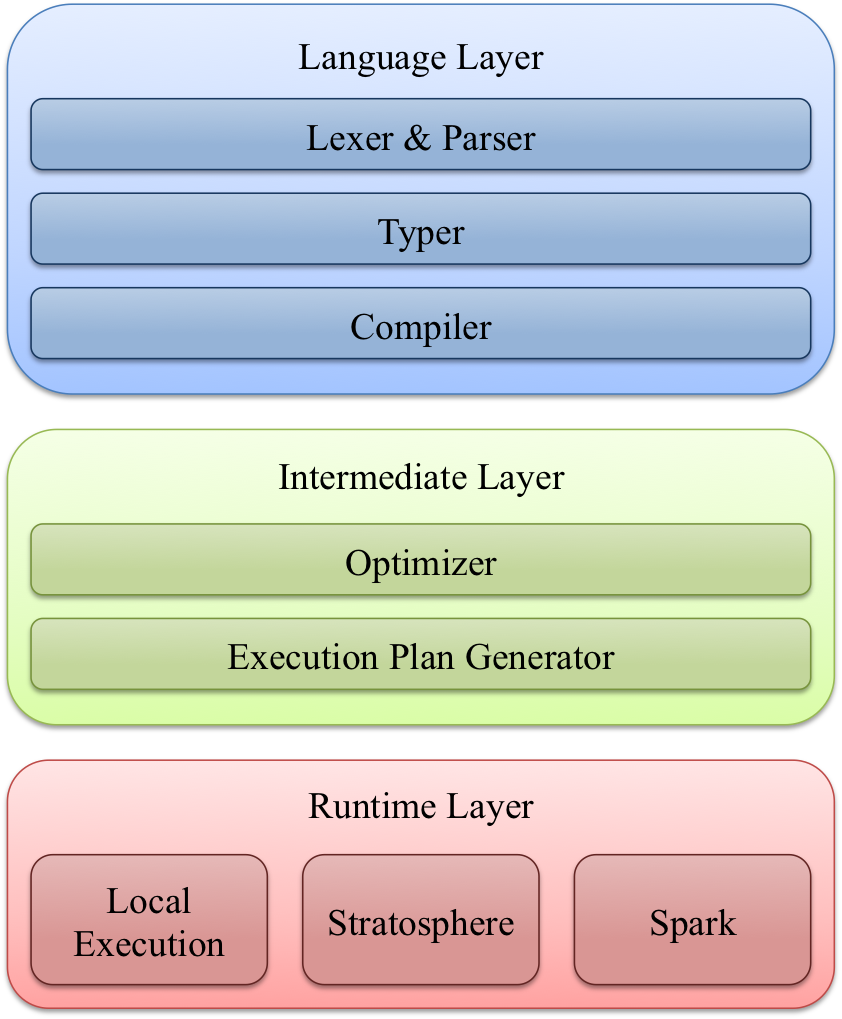
\includegraphics[height=0.175\paperheight]{images/systemArchitecture.png}
\caption{The layered system architecture of Gilbert. The language layer is responsible for parsing, typing and compiling the given Matlab code. The intermediate layer facilitates high-level optimization strategies. The runtime layer is responsible for executing the specified program in parallel.}
\label{fig:systemArchitecture}
\end{figure}

As a solution we propose Gilbert, a distributed sparse linear algebra environment. Gilbert provides a Matlab-like language for distributed sparse linear algebra operations. It has a layered architecture, which is shown in Figure \ref{fig:systemArchitecture}. The first layer is the language layer. It contains all functionality to parse the given Gilbert code and to compile it into an intermediate representation (IR). The second layer is the intermediate layer and it receives the IR of the Gilbert code. The intermediate format is the ideal representation to apply language independent high-level transformations. The Gilbert optimizer applies several algebraic optimizations prior to the generation of the execution plan. The execution plan generator translates the optimized IR into a specific execution plan, depending on the selected execution engine. Once the program has been translated into an execution engine's specific plan, it is executed on the respective back end. 

Our main contributions are:
\begin{itemize}
 \item Gilbert allows to write MATLAB-like code for sparse linear algebra and execute it on massively parallel dataflow systems.
 \item Its expressiveness allows to quickly develop scalable algorithms to analyze web-scale data.
 \item We introduce a novel fixed-point operator which replaces loops by recursion and can be efficiently parallelized.
 \item Furthermore, we demonstrate that dataflow optimizers can be used to automatically select an good matrix multiplication strategy. 
\end{itemize}
%Gilbert provides a Matlab-like language for distributed sparse linear algebra operations. %Being such a system, it comprises the complete stack of functionalities necessary to implement a programming language. At first, the system has to divide the given source code into tokens. These tokens are parsed and an abstract syntax tree (AST) is created. In order to generate the intermediate representation (IR), type information is needed for all expressions. This information is extracted by the typing system. Knowing the types, the compiler can translate the Gilbert program into its IR. The IR is well suited to apply high-level transformations to the program. At last, the execution plan generator translates the IR into an execution plan which can be executed in parallel. %The layered system architecture is shown in \cref{fig:systemArchitecture}. 

%%It has a layered architecture. The first layer is the language layer. It contains all functionality to parse the given Gilbert code and to compile it into an intermediate representation (IR). The second layer is the intermediate layer and it receives the IR of the Gilbert code. The intermediate format is the ideal representation to apply language independent high-level transformations. The Gilbert optimizer applies several algebraic optimizations prior to the generation of the execution plan. The execution plan generator translates the optimized IR into a specific execution plan, depending on the selected execution engine. Once the program has been translated into an execution engine's specific plan, it is executed on the respective back end.

%\begin{figure}[t!]
% \centering
% 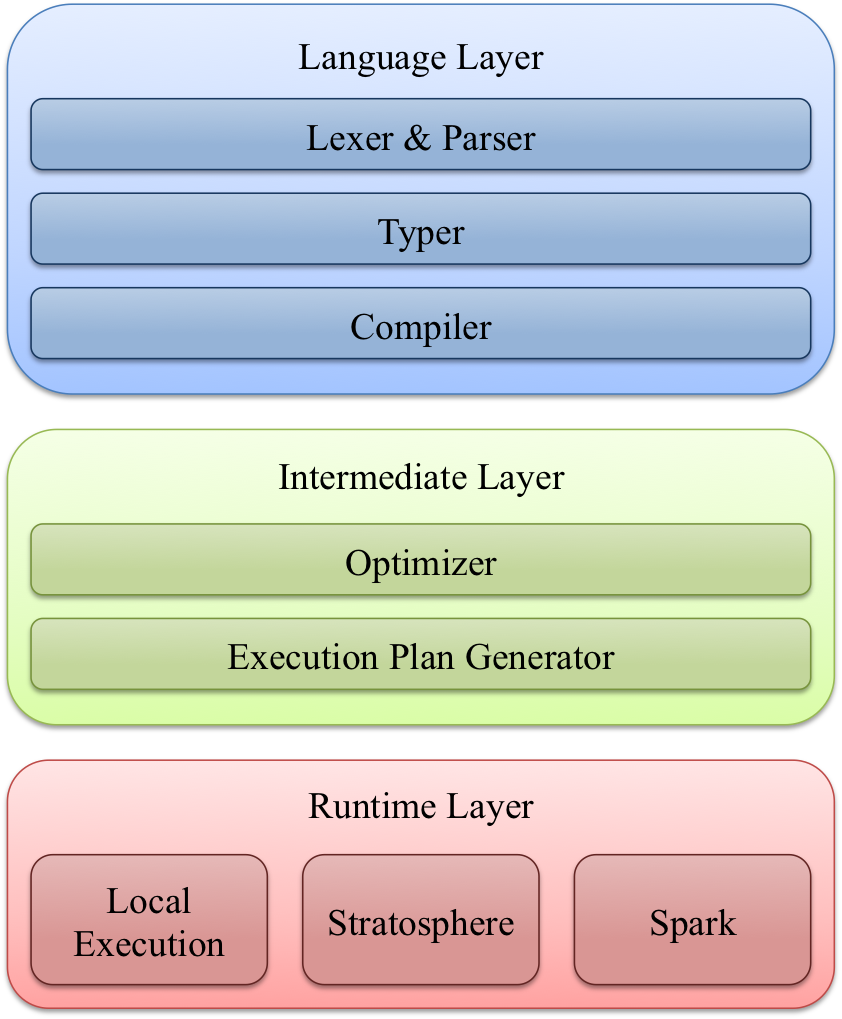
\includegraphics[height=0.175\paperheight]{images/systemArchitecture.png}
% \caption{The layered system architecture of Gilbert. The language layer is responsible for parsing, typing and compiling the given Matlab code. The intermediate layer facilitates high-level optimization strategies. The runtime layer is responsible for executing the specified program in parallel.}
% \label{fig:systemArchitecture}
%\end{figure}

%%\textbf{Language Layer}. The language layer contains all the logic for translating Gilbert source code into the intermediate representation, see the subsequent section for more details. %Gilbert's supported language and its features is described in \cref{sec:gilbertLanguage}.
%%The resulting AST is attributed with type information by the typing system. The typer makes use of the Hindley-Milner algorithm to automatically infer types.%, as it is described in~\cref{sec:hmInference}. 
%%The type information enriched AST is then translated into a front end independent representation of linear algebra operations, namely the IR. The format Gilbert uses to represent linear algebra operations in a generalized format is described in Section~\ref{sec:intermediaterepresentation}.

%%\textbf{Intermediate Layer}. The intermediate layer contains the optimizer and the execution plan generator. The optimizer applies the optimizations described in Section~\ref{sec:gilbertOptimizer} to IR of the Gilbert program. Then the IR is translated into the execution engine's specific format. The linear algebra operations are translated into a dataflow graph as explained in Section~\ref{sec:LinearAlgebraOperations}. The system supports Flink and Spark as parallel execution engines.

The rest of this paper is structured as follows. %In \ref{sec:overview} we give an overview of Gilbert.
%Then, 
In \Cref{sec:gilbertFeatures}, Gilbert's language and its features are described.
\Cref{sec:gilbertRuntime} presents how linear algebra operations are mapped to a dataflow system. Gilbert's performance and scalability is evaluated in \Cref{sec:evaluation}.
Related work is covered in \Cref{sec:relatedWork} before the work is concluded in \Cref{sec:conclusion}.